\chapter{ Системы отображения информации}

По способу отображения информации индикаторные устройства приборов разделяют на \textit{шкальные} и \textit{цифровые}.

\textit{В шкальных индикаторных устройствах} значения измеряемой величины представляют в виде взаимного смещения одного или нескольких подвижных элементов в виде шкалы и указателя. Шкалу выполняют как совокупность отметок (штрихов), расположенных по прямой, дуге или окружности и соответствующих ряду последовательных значений измеряемой величины. Указатель выполняют в виде стрелки, индекса со штрихом или светового пятна, которые занимают определенное положение относительно отметки шкалы и показывают деление шкалы, соответствующее значению измеряемой величины. Шкальные индикаторные устройства находят широкое применение в современных приборах благодаря простоте конструкции, компактности, большой надежности и достаточно высокой точности отсчета.

\textit{В цифровых индикаторных устройствах} результат отсчета измеряемой величины представляется в виде числа (обычно десятичной системы). Цифровой отсчет имеет ряд важных достоинств: отсутствие субъективных погрешностей, удобство отсчета на большом расстоянии и при большем угле наблюдения, малая утомляемость оператора, возможность автоматической регистрации результатов измерений в измерительных системах и автоматизированных системах управления.

\section{Шкальные индикаторные устройства}

В зависимости от назначения и предъявляемых технических требований в индикаторных устройствах используют неподвижные или подвижные круговые (дуговые) и прямолинейные шкалы в сочетании с подвижными или неподвижными указателями. Наибольшее распространение имеют круговые неподвижные шкалы при подвижном указателе. Отметки на шкалах разделяют на три вида (ГОСТ~5365-73):
\begin{itemize}
\item главные, обозначающие целые числа;
\item средние, обозначающие $ \dfrac{1}{2} $  или $ \dfrac{1}{5} $ часть главного деления;
\item малые, обозначающие $ \dfrac{1}{5} $ или $ \dfrac{1}{10} $ часть главного деления.
\end{itemize}

\textit{Делением шкалы} называют участок шкалы, ограниченный соседними отметками (штрихами). Линейное или угловое расстояние между центрами двух соседних отметок шкалы называют длиной деления шкалы.

\textit{Масштаб шкалы} есть отношение длины деления шкалы к измеряемой величине, соответствующей этому делению.

\textit{Ценой деления шкалы} называют число единиц измеряемого параметра, приходящееся на одно деление шкалы.

\begin{figure}[h!]
	\caption{ Зависимость между смещением указателя и значением измеряемой величины }
	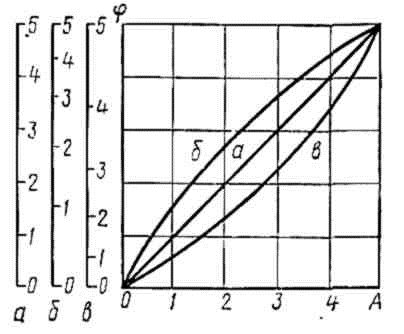
\includegraphics[width=0.4\textwidth]{12scale.png}
	\label{pic:12scale}
\end{figure}

По виду зависимости между смещением указателя $ \varphi $ и значением измеряемой величины $ А $ различают равномерные и неравномерные шкалы. Равномерные шкалы (рис.~\ref{pic:12scale}~а) обладают постоянной чувствительностью; их применяют в тех случаях, когда требуется получить одинаковую по всей шкале абсолютную погрешность измерений. Неравномерные шкалы (рис.~\ref{pic:12scale}~б,~в) имеют криволинейную характеристику и непостоянную чувствительность. Их применяют в тех случаях, когда требуется получить постоянную по всей длине шкалы относительную погрешность измерений. 

\begin{figure}[h!]
	\caption{ Конструктивные формы концов (а) и сечений(б) указателей }
	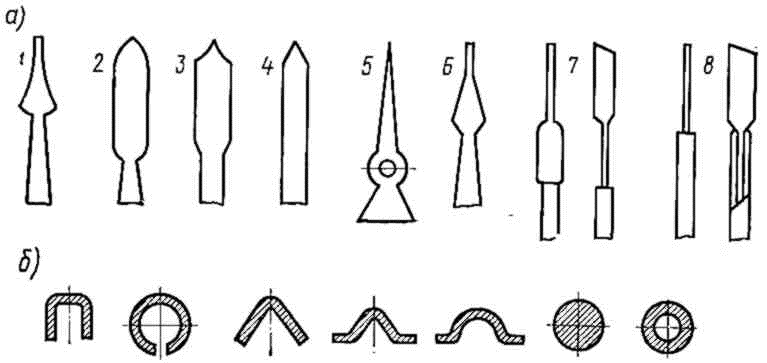
\includegraphics[width=0.6\textwidth]{12end.png}
	\label{pic:12end}
\end{figure}

На рис.~\ref{pic:12end}~а изображены основные конструктивные формы концов, а на рис.~\ref{pic:12end}~б~--- сечения указателей. Часто применяют указатели с ножевидными концами (6, 7, 8), толщина ножа у которых обычно равна 0,1$ \ldots $0,2~мм, что соответствует толщине штриха шкалы. В индикаторных устройствах, находящихся на сравнительно большом расстоянии от оператора (1$ \ldots $2~м и более), ставят стержневые (4), мечевидные (5) и копьевидные (1, 2, 3) указатели. Указывающий конец стрелки в любом случае не должен быть толще самой тонкой отметки на шкале, а длину стрелки выбирают так, чтобы ее конец перекрывал $ \dfrac{1}{4} \ldots  \dfrac{3}{4}$ высоты наименьшей отметки на шкале. Форма сечения указателя должна быть такой, чтобы момент сопротивления площади поперечного сечения был наибольшим при наименьшей массе и моменте инерции самого указателя относительно оси его вращения. Противоположный конец указателя должен уравновешивать его указывающую часть. Для увеличения чувствительности индикаторного устройства и устранения параллакса  применяют световые указатели (рис.~\ref{pic:12lightend}). В таких устройствах штрих 2 после одно- или многократного отражения от зеркала 3 посредством оптической системы 1 проецируется на шкалу 4.

\begin{figure}[h!]
	\caption{ Световой указатель }
	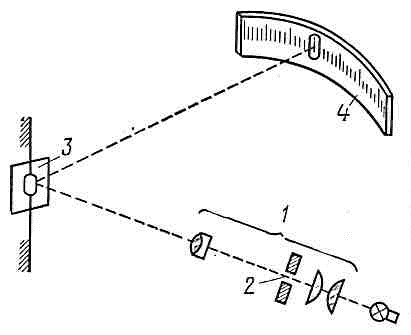
\includegraphics[width=0.65\textwidth]{12lightend.png}
	\label{pic:12lightend}
\end{figure}

В качестве исходных данных для расчета шкал используют: $ A $ -- количество единиц или диапазон изменения измеряемого параметра; $ \Delta A $ -- абсолютную погрешность измерения параметра; рабочую длину $ L $ или угол $ \theta $ оцифровки шкалы (для линейных и круговых шкал соответственно). 

При указанных заданных величинах цена деления шкалы $ a $, число делений шкалы $ n $, расчетное значение длины $ L_p $ шкалы, расчетный диаметр $ d_p $ шкалы соответственно равны:
\[ a = 2\Delta A, \, n = \dfrac{A}{a}, \, L_p = n[p], \, d_p = \dfrac{2n[b]}{\theta},  \]
где $ \delta A $ -- относительная погрешность измерения; $ [b] $ -- 1,5$ \ldots $4,0~мм~-- допустимая длина деления шкалы, которую выбирают в зависимости от условий эксплуатации индикаторного устройства. 

В приборных устройствах часто применяют многошкальные индикаторные устройства. Двухшкальное устройство состоит из шкалы грубого отсчета диаметром $ d_\text{г} $ и числом делений $ n_\text{г} $ и шкалы точного отсчета с соответствующими параметрами $ d_\text{т} $ и $ n_\text{т} $.

Цена деления шкалы точного отсчета:
\[ a_\text{т} = 2\Delta A.  \]

Общее число делений обеих шкал:
\[ n = \dfrac{A}{a_\text{т}} = n_\text{т}n_\text{г}. \]

Для шкалы точного отсчета обычно число делений:
\[ n_\text{т} = 10;\,50;\,100. \]

Число делений шкалы грубого отсчета:
\[ n_\text{г}= \dfrac{n}{n_\text{т}}, \, \text{цена её деления} \, a_\text{г} = \dfrac{A}{n_\text{г}} = a_\text{т}n_\text{т}. \]

Длина и расчетный диаметр шкалы грубого отсчета:
\[ L_\text{р.г.} = n_\text{г}[b]; \, d_\text{р.г.} = \dfrac{2n_\text{г}[b]}{\theta_\text{г}} \leq d_\text{г}. \]

Параметры шкалы точного отсчета:
\[ L_\text{р.т.} = n_\text{т}[b]; \, d_\text{р.т.} = \dfrac{2n_\text{т}[b]}{\theta_\text{т}} \leq d_\text{т}. \]

Коэффициент умножения масштаба шкалы равен передаточному отношению между шкалами точного и грубого отсчетов:
\[ i_\text{тг} = \dfrac{\theta_\text{т}}{\theta_\text{г}} = n_\text{г}^{-1} \]

В качестве примера на рис.~\ref{pic:12device} показано устройство, в котором шкала грубого (ШГО) отсчета имеет 72 равных деления с ценой деления 5$ ^\circ $ и углом поворота 360$ ^\circ $, а шкала точного отсчета (ШТО)~--- 100 равных делений. За один полный оборот шкалы точного отсчета шкала грубого отсчета повернется на 5$ ^\circ $ (одно деление ШГО). Цена деления ШТО равна 3$ ' $.

\begin{figure}[h!]
	\caption{ Пример ШТО и ШГО }
	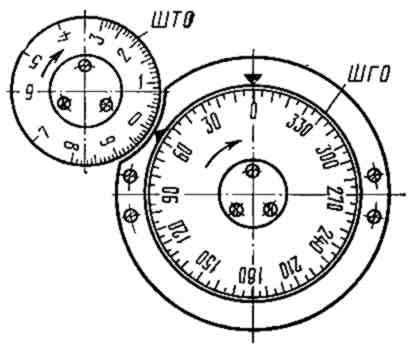
\includegraphics[width=0.4\textwidth]{12device.png}
	\label{pic:12device}
\end{figure}

\section{ Цифровые устройства отображения информации }
По способу воспроизведения цифр цифровые отсчетные устройства разделяют на четыре группы:
\begin{enumerate}
\item Цифры выполняют целиком в виде заранее известной фигуры в соответствии с принятыми шрифтами (например, цифра~5 на рис.~\ref{pic:12digital}~а). Такое изображение цифры является самым удобным и совершенным для визуального снятия отсчета.
\item Цифры синтезируют из отдельных полос-сегментов (рис.~\ref{pic:12digital}~б). При различных комбинациях светящихся сегментов на одном знакоместе получают изображения разных цифр. Для упрощенного воспроизведения арабских цифр от~0 до 9 используют семь сегментов (рис.~\ref{pic:12digital}~б). Иногда на семисегментном индикаторе отображают и некоторые буквы. Часто цифры в семисегментном индикаторе имеют наклон. Это делается производителем индикаторов для удобства размещения на них десятичной точки.
\item Цифры набирают из отдельно светящихся точечных элементов в виде мозаики (рис.~\ref{pic:12digital}~в). Каждая точка обслуживает одну или несколько цифр. На некотором расстоянии от приборной доски или панели при соответствующей коммутации набор точек воспринимается глазом оператора как сплошная светящаяся цифра благодаря иррадиации зрения.
\item Цифры воспроизводят на экране быстро перемещающимся световым пятном. Если светящаяся точка обходит полный контур цифры за 0,05~с, что соответствует времени сохранения глазом информации, то оператор воспринимает сплошную цифру благодаря инерции зрения.
\end{enumerate}

\begin{figure}[h!]
	\caption{ Цифровые устройства отображения информации }
	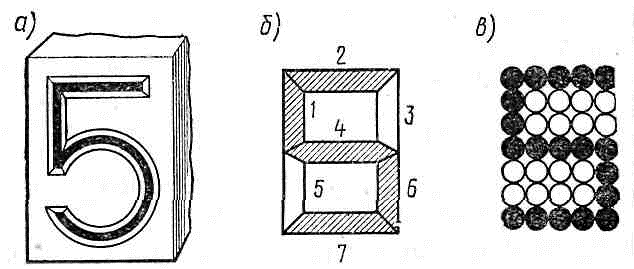
\includegraphics[width=0.6\textwidth]{12digital.png}
	\label{pic:12digital}
\end{figure}

Использование семисегментных индикаторных устройств позволяет сформировать все десятичные цифры и часть букв. Однако не все символы могут быть отображены на этом индикаторе. Для отображения всех цифр, символов и букв алфавита в настоящее время используются более сложные многосегментные и матричные индикаторные устройства. 

\textit{Матричный индикатор} --- устройство отображения информации, элементы отображения которого сгруппированы по строкам и столбцам. Матричный индикатор предназначен для отображения информации в виде букв, цифр, математических и специальных знаков, знаков препинания и др. символов. Матричным индикатором считается устройство, объединенное в законченном конструктиве~--- корпусе. В отличие от матричных мониторов, дисплеев или экранов, матричным индикатором принято считать устройство с относительно небольшим количеством пикселей, или устройство, предназначенное для вывода одного или нескольких символов, хотя граница довольно размыта. 

Исходя из определения, матричный индикатор имеет два и более рядов и два и более столбцов однотипных элементов отображения (точек, пикселей) с индивидуальным управлением. Практическое применение имеют матричные индикаторы 5х7, 5х8, 8х8 и более пикселей. Форма пикселя обычно~-- круглая, но встречаются квадратные, а также структурированные пиксели. Наиболее распространены матричные индикаторы 5x7. Пример изображения на таком индикаторе буквы S приведён на рис.~\ref{pic:12S}.

\begin{figure}[h!]
	\caption{ Пример изображения буквы S на матричном индикаторе 5x7 }
	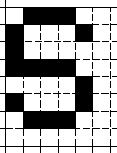
\includegraphics[width=0.2\textwidth]{12S.png}
	\label{pic:12S}
\end{figure}

Для отображения цифровой информации можно воспользоваться различными индикаторами, такими как малогабаритные лампочки накаливания, газоразрядные индикаторные лампы, электролюминисцентные, катодолюминисцентные, светодиодные и жидкокристаллические индикаторы. Рассмотрим кратко каждый из этих видов индикаторов.

\textit{Малогабаритные лампочки накаливания} не отличаются надёжностью, так как при включении питания через них протекает значительный ток, в результате воздействия которого на нить накаливания лампа может выйти из строя. Кроме того они боятся ударов. Эти причины, а также большой потребляемый ток привели к тому, что в настоящее время эти индикаторы практически не используются.

В \textit{газоразрядных индикаторах} используется свечение газа под действием электрического тока. Все газоразрядные индикаторы работают в режиме тлеющего разряда с холодным катодом. Газоразрядные лампы в отличие от ламп накаливания управляются не напряжением, а током. Отличительная особенность этих ламп состоит в том, что изображения различных цифр одного разряда создаются цельными на одном знакоместе. Для этого внутри баллона лампы располагают несколько светящихся катодов и один анод в виде тонкой редкой сетки. Катоды выполняют в виде отдельных цельных цифр и располагают стопкой один за другим так, что образуется пакетная конструкция лампы. При наличии управляющего напряжения на аноде и одном из катодов между ними в газовой среде возникает тлеющий разряд, вид свечения которого внутри баллона лампы имеет форму катода-цифры. Смена изображения цифр на одном знакоместе осуществляется последовательной коммутацией напряжения на различные катоды.

\textit{Электролюминесцентные цифровые устройства} основаны на использовании явления свечения кристаллических веществ (электролюминофоров) при возбуждении их электрическим полем. Индикаторная ячейка состоит из прозрачной стеклянной пластинки, с внутренней стороны которой нанесён тонкий проводящий слой, затем слой люминофоров, а затем проводники-сегменты. Электролюминофоры возбуждаются и светятся при подаче на электроды переменного управляющего напряжения.

\textit{Катодолюминесцентные цифровые устройства} представляют собой электровакуумные триоды в стеклянном баллоне, у которых аноды выполнены в виде отдельных сегментов, покрытых катодолюминофорами. В стеклянном баллоне в вакууме находятся также катод прямого накала и сетка для управления индикатором. Работа катодолюминесцентных устройств основана на способности люминофоров преобразовывать кинетическую энергию электронов в световую энергию. При прохождении тока через нить накала она нагревается и испускает электроны. Сетка и включенные аноды имеют, как правило, одинаковый положительный потенциал, так что электроны, приобретая некоторую скорость, пролетают по инерции сетку и достигают анода. Под действием падающих электронов нанесенный на анод люминофор начинает светиться. При отсутствии на аноде положительного напряжения поток электронов тормозится, его энергия мала и люминофор не светится. Поэтому в каждый момент времени светится тот анод-сегмент, на который подано напряжение, а конфигурация цифры определяется набором светящихся сегментов.

В настоящее время газоразрядные индикаторные лампы, а также электролюминисцентные и катодолюминисцентные индикаторы практически не используются.

\section{Цифровые устройства на светоизлучающих диодах}

Полупроводниковые источники излучения оптического диапазона спектра способны эффективно преобразовывать электрическую энергию в световую. Принцип действия светоизлучающих диодов основан на инжекционной люминесценции: свечение возникает при пропускании электрического тока через границу двух слоев полупроводника с $ p-n $--проводимостью. Светодиоды для видимого и ближнего инфракрасного излучения изготовляют из монокристаллических материалов типа $ A^{III}B^{V} $: фосфида галлия ($ GaP $), арсенида галлия ($ GaAs $) и более сложных соединений $ GaAs_{x-1}P_x $, $ Ga_{1-x}Al_{х}As $, где $ x $~-- доля содержания того или другого элемента в соединении.

Способом вытягивания из раствора изготовляют кристаллы $ GaP $ достаточно больших размеров. Используя $ GaP $ с различными присадками, получают светодиоды разных цветов излучения. Так, для получения красного излучения $ GaP $ легирует цинком и кислородом, а для получения зеленого цвета~--- азотом. Светодиоды на $ GaAs $ дают излучение в инфракрасной области спектра. Для преобразования этого излучения в излучение видимого диапазона используют люминофоры, в частности синтезированные на основе бария и лантана. Люминофорное покрытие может иметь различный цвет; широкая цветовая гамма излучения светодиода с люминофором расширяет возможности создания и применения многоцветных цифровых индикаторных устройств. В сложных полупроводниковых соединениях цвет излучения изменяется с изменением параметра $ x $. 

Например, фосфид арсенида галлия $ GaAsP $ обладает достаточно высокой эффективностью излучения в красном диапазоне спектра. Светоизлучающие диоды выполняют и на основе карбида кремния $ SiC $, который дает излучение в желтой области спектра, но не обладает высокой эффективностью. Диоды на основе $ SiC $ имеют достаточно хорошую температурную стабильность параметров, что позволяет эксплуатировать их при температуре до $ 300\ldots 400$~$ ^\circ $C. 

Светодиоды работают при низких рабочих напряжениях и малой потребляемой мощности, имеют малые габариты и массу, обладают высокой скоростью переключения. Так, например, быстродействие светодиодов на основе $ SiC $ и $ GaAlAs $ составляет единицы наносекунд. 

Цифровые индикаторные устройства на светодиодах применяют в разнообразных индикаторных устройствах: электронных часах с цифровым отсчетом времени; карманных ЭВМ и калькуляторах; в индикаторных устройствах приборов самолетов и космических кораблей; в средствах визуального считывания информации и контроля при дистанционном управлении.

Наиболее распространены плоская (рис.~\ref{pic:12plan}~а) и полусферическая (рис.~\ref{pic:12plan}~б) конструкции светодиодов.

\begin{figure}[h!]
%	\caption{ Конструкция светодиодов:\\ плоская (а) и полусферическая (б) }
	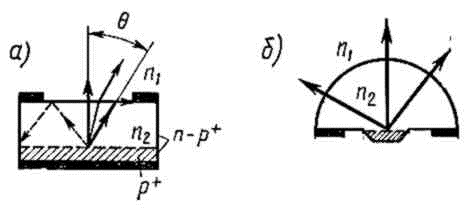
\includegraphics[width=0.5\textwidth]{12plan.png}
	\label{pic:12plan}
\end{figure}

В плоских конструкциях из кристалла выходят только те лучи, которые составляют с нормалью угол:
\[ \theta \leq \arcsin\dfrac{n_1}{n_2}, \]
где $ n_1 $ и $ n_2 $ -- показатели преломления сопряженных сред. Для $ GaAs $ и $ GaP $ это конус с углом при вершине не более 35$ ^\circ $. Остальные лучи имеют полное внутреннее отражение на границе раздела сред с различными показателями преломления и не выходят из кристалла. Плоские конструкции наиболее удобны, но они обладают малой эффективностью и имеют узкую диаграмму направленности излучения. 

Геометрические размеры светодиодов полусферической конструкции выбирают таким образом, чтобы все излучение, распространяющееся по различным направлениям полностью выходило наружу. Эффективность полусферической конструкции светодиода приблизительно в 10 раз выше эффективности плоской конструкции, но она дороже и сложнее в изготовлении.

Так как светодиоды являются миниатюрными твердотельными источниками излучения и имеют малую поверхность излучения, то при разработке цифровых индикаторных устройств на светодиодах для увеличения размеров светового изображения используют линзы, отражатели или фоконы (фокусирующий конус). 

Конструктивно линза может быть вмонтирована в корпус источника излучения (рис.~\ref{pic:12reflector}~а) или располагаться непосредственно на кристалле (рис.~\ref{pic:12plan}~б), выполняя роль прозрачного корпуса. Для изготовления прозрачного сферического корпуса могут быть использованы пластмасса, нейтральные и поляризационные фильтры, цветное стекло для повышения контраста изображения, люминесцентные материалы для преобразования инфракрасного излучения в видимое. 

Роль линзы может выполнять капля смолы с показателем преломления $ n_3 $, нанесенная на плоский кристалл светодиода (рис.~\ref{pic:12reflector}~б). Показатель преломления эпоксидной смолы выбирают между показателями преломления воздуха и материала кристалла, что уменьшает потери световой энергии на отражение. При использовании линзы кажущийся размер светящейся площадки светодиода в 1,5$ \ldots $2 раза больше фактической. При применении рефлектора (отражателя)~3 (рис~\ref{pic:12reflector}~в) для увеличения размеров светящейся поверхности~1 размер светового изображения зависит от формы отражающей поверхности~2, отношения высоты отражателя к его ширине.

\begin{figure}[h!]
	\caption{ Светодиоды:  }
	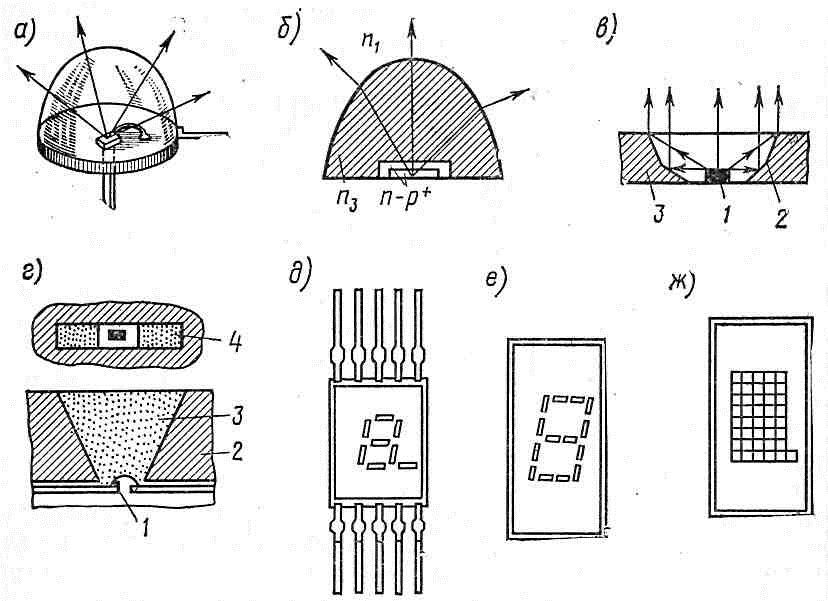
\includegraphics[width=1\textwidth]{12reflector.png}
	\label{pic:12reflector}
\end{figure}

В большинстве случаев отражатели в поперечном сечении имеют вид прямоугольника (полосы), который выполняет роль сегмента в цифро-синтезирующих устройствах. В некоторых конструкциях полоска-сегмент образуется отражением излучения от трех светодиодов, установленных в одном отражателе. Темные участки в пределах полосы малы и практически не заметны для глаза на расстоянии до приборной доски или панели, где расположено индикаторное устройство. При использовании конической призмы-фокона (рис.~\ref{pic:12reflector}~г) светящееся изображение~4 также имеет вид полосок-сегментов. Призма~3 может быть изготовлена из цветного оргстекла, которое одновременно служит и фильтром, повышающим контраст изображения. При использовании указанных устройств обеспечивается видимый размер светящихся цифр 1,5$ \ldots $3 и 25$ \ldots $50 мм, что позволяет оператору считывать цифровую информацию на расстоянии 3$ \ldots $10~м соответственно.

Цифровые индикаторные устройства на светодиодах выполняют в основном сегментными и матричными. На рис.~\ref{pic:12reflector}~д,~е показаны плоские конструкции, состоящие из 8 и 14 сегментов соответственно. Они обеспечивают большой угол наблюдения и могут быть установлены и закреплены на приборных досках и панелях. Каждый сегмент состоит из нескольких, например трех, светодиодов, соединенных между собой последовательно. В матричных цифровых устройствах для создания изображения цифр в большинстве случаев используют 5 и 7 отдельных светодиодов как точечных источников света (рис.~\ref{pic:12reflector}~ж). Изображение цифры создается избирательным возбуждением отдельных диодов, что обеспечивает высокую универсальность, качество и надежность изображения большую, чем в сегментных устройствах.

\begin{flushleft}
\textbf{Светотехнические характеристики}
\end{flushleft}

Основной светотехнической характеристикой светодиода является сила излучаемого им света $ I $~--- кандела. К светотехническим характеристикам также относятся длина волны излучаемого цвета и диаграмма направленности. Современные светодиоды, применяемые в экранах имеют следующие длины волн: синий 430~-- 470~нм, зеленый 515~-- 530~нм, красный 630~-- 670~нм. 

Выходная диаграмма направленности светового потока формируется как формой рефлектора, так и формой корпуса светодиода. Варьируя параметры рефлектора и корпуса можно создавать различные диаграммы направленности шириной от 4-5 до 160$ ^\circ $. Более того, возможно создание диаграмм направленности с различной шириной по вертикали и горизонтали, например, 120$ ^\circ $ по горизонтали и 60$ ^\circ $ по вертикали (т.н. овальные светодиоды). 

\begin{flushleft}
\textbf{Светодиодный экран}
\end{flushleft}

В светодиодном экране в качестве источника света используются полупроводниковые светодиоды. Светодиоды имеют очень большой ресурс работы в непрерывном режиме работы (до 100 тыс. часов), поэтому замена модулей довольна редка, что значительно снижает затраты на обслуживание.

Светодиодные экраны по принципу построения делятся на \textit{кластерные} и \textit{матричные}.

В \textit{кластерных экранах} каждый пиксель, содержащий от трех до нескольких десятков светодиодов, объединён в отдельном светоизолированном корпусе, который залит герметизирующим компаундом. Такой конструктивный элемент называется кластером.

Кластеры, образующие информационное поле экрана, закреплены при помощи винтов на лицевой поверхности экрана. От каждого кластера отходит жгут проводов, подключаемый, посредством электрического разъема, к соответствующей схеме управления (плате). Такой способ построения полноцветных светодиодных экранов постепенно отмирает, уступая место более технологичному матричному принципу.

В \textit{матричных светодиодных экранах} кластеры и управляющая плата объединены в единое целое~--- матрицу, то есть на управляющей плате смонтированы и светодиоды и коммутирующая электроника, которые залиты герметизирующим компаундом. В зависимости от размера и разрешения экрана, количество светодиодов, составляющих пиксель, может колебаться от трех до нескольких десятков. А распределение количества светодиодов по цветам в пикселе изменяется от типа применяемых светодиодов в интересах соблюдения баланса белого.

Диаграмма направленности экрана формируется каждым светодиодом. Для того чтобы диаграмма направленности экрана в целом соответствовала диаграмме направленности диодов, необходимо использовать светодиоды разных цветов свечения с идентичными конструктивными параметрами. Светодиоды должны устанавливаться в экран с минимально возможными отклонениями по высоте и углам наклона относительно осевой линии. Для овальных светодиодов также важно не допускать поворотов относительно оси. Нарушение этих требований приводит к разбросу диаграмм направленности различных светодиодов. При наблюдении экрана под достаточно большими к нормали углами такой разброс выражается в появлении на изображении аномально ярких точек различных цветов. 

Как правило, для экранов, используемых внутри помещений, используются светодиоды с достаточно широкой диаграммой направленности, например, 120х60$ ^\circ $. Для уличных экранов используют светодиоды с более узкой диаграммой направленности, например, 70х30$ ^\circ $. Такое различие объясняется разными условиями наблюдения. Возможность обмена ширины диаграммы направленности (путем замены одного типа светодиодов на другой) на яркость является отличительной чертой светодиодных экранов. При прочих равных условиях, сужение диаграммы со 120х60$ ^\circ $ до 70х30$ ^\circ $ позволяет повысить яркость в 3-4 раза.  

Светодиодные светофоры имеют ряд существенных преимуществ по сравнению со светофорами на основе ламп накаливания. Ресурс светодиодных модулей составляет более чем 100000 часов и намного превышает ресурс ламп накаливания, что заметно снижает расходы на обслуживание и эксплуатацию. При этом потребление электроэнергии составляет 10-20\% от электропотребления лампового светофора. Все это делает установку светодиодных светофоров экономически выгодной и позволяет быстро окупить расходы на переоборудование. Качественное отличие светодиодных светофоров в том, что в них полностью отсутствует фантомный эффект, т.е. не возникает иллюзии одновременного включения сигнала всех трех секций светофора при солнечной засветке, что повышает безопасность дорожного движения.

\section{Цифровые устройства на жидких кристаллах}

Жидкокристаллические индикаторы появились еще в 70-е годы и стали широко применяться в качестве средств отображения информации~(СОИ). ЖК-индикаторы~--- пассивные устройства. Они не генерируют свет и требуют дополнительной подсветки, сами же выполняют роль модулятора, работая в режиме пропускания или отражения света.

Жидкие кристаллы (ЖК) представляют собой органические жидкости, имеющие удлиненные стержнеобразные молекулы. Различают ЖК трех типов (рис.~\ref{pic:12liquid}): \textit{смектические}, \textit{нематические} и \textit{холестерические}.

\textit{В смектических ЖК} сильно вытянутые молекулы располагаются слоями одинаковой толщины, близкой к длине молекул. Ориентированы молекулы параллельно друг другу. 

\textit{У нематических ЖК} отсутствует слоистая структура, а молекулы также ориентированы параллельно друг другу своими длинными осями. 

\textit{Холестерические ЖК} имеют структуру слоистую, но в каждом слое молекулы вытянуты в некотором преимущественном направлении.

\begin{figure}[h!]
%	\caption{ Типы жидкокристаллических индикаторов:\\ а -- смектические; б -- нематические; в -- холестерические }
	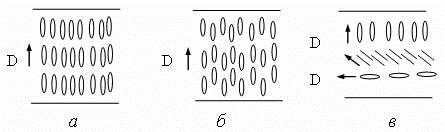
\includegraphics[width=1\textwidth]{12liquid.png}
	\label{pic:12liquid}
\end{figure}

Ориентация отдельной молекулы ЖК подвергается непрерывным тепловым флюктуациям, однако в любой точке жидкости существует средняя ориентация, характеризуемая единичным вектором, называемым директором $ D $. Когда ЖК-вещество занимает большой объем, то в молекуле появляются области с независимыми ориентациями директора. Для придания одинаковой ориентации во всем рабочем пространстве ЖК заключают в узкое (несколько десятков микрометров) пространство между подложками. В результате специфическая ориентация молекул ЖК определяется и соседними молекулами, и граничной поверхностью подложки. Ориентирующее действие достигается напылением на подложки тонких пленок $ SiO_2 $.

Молекулы ЖК представляют собой индивидуальные диполи. Ориентация молекул может меняться в результате различных электрогидродинамических эффектов, обусловленных протеканием даже небольшого тока или под действием электрического поля.

Конструкция элементарной ячейки ЖК-индикатора проста и содержит две стеклянные пластины, имеющие на внутренней стороне прозрачное проводящее покрытие. Между пластинами залит ЖК. Толщина ЖК лежит в пределах от 6 до 25~мкм. Такая конструкция по сути представляет собой плоский конденсатор. При отсутствии напряжения на ячейке ЖК-вещество однородно и прозрачно.

В настоящее время распространены ЖК-индикаторы на основе эффекта \textit{динамического рассеивания}, а также ЖК-индикаторы, использующие \textit{полевой твист-эффект} и \textit{эффект типа <<гость-хозяин>>}.

\textit{Эффект динамического рассеяния} состоит в том, что при приложении электрического поля к тонкому слою жидкокристаллического вещества, заключенному между двумя стеклянными пластинками, происходит разрушение упорядоченной структуры жидких кристаллов, т.е. ЖК теряет оптическую однородность, что вызывает диффузное рассеяние света в этой области. В результате прозрачный жидкокристаллический слой становится мутным и при внешнем освещении возникает контраст между возбужденным участком жидкости кристаллов и невозбужденным (фоном). При снятии внешнего электрического поля первоначальная структура жидких кристаллов восстанавливается и указанный контраст исчезает.

Рассмотрим подробнее индикаторы, использующие полевой твист-эффект. Работа ячейки со скрещенными поляризатором~П и анализатором~А показана на рис.~\ref{pic:12liquid1}.

\begin{figure}[h!]
%	\caption{ Работа ЖК-индикатора на твист-эффекте при напряжениях:\\ а -- нулевом; б -- превышающем пороговое }
	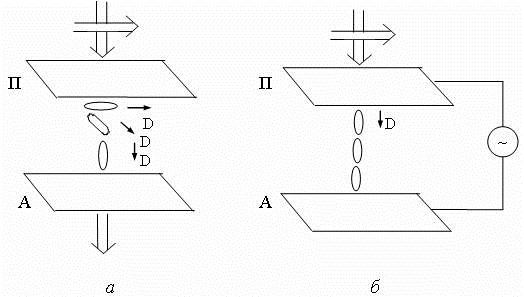
\includegraphics[width=1\textwidth]{12liquid1.png}
	\label{pic:12liquid1}
\end{figure}

В отсутствие напряжения питания на ячейке молекулы ЖК закручены приблизительно на 90$ ^\circ $ благодаря ориентирующему действию подложек П и А, причем молекулы ЖК упорядочены послойно определенным образом между этими подложками. Ориентация каждого слоя ЖК плавно изменяется от верхнего к нижнему слою, формируя спираль. Поляризатор~-- это оптический элемент, пропускающий свет, поляризованный в одном направлении, и гасящий свет, поляризованный в противоположном направлении, в зависимости от ориентации поляризатора.

Жидкокристаллические индикаторы (ЖКИ) управляют отражением и пропусканием света для создания изображений цифр, букв, символов. Свет, падающий сверху, поляризуется таким образом, что его вектор поляризации совпадает с направлением директора $ D $ у верхней подложки. При прохождении через ЖК плоскость поляризации света вращается (как директор у молекул ЖК) и свет проходит через анализатор. Под действием электрического поля молекулы ЖК переориентируются параллельно полю. Этот процесс называется твист-нематическим полевым эффектом (twisted nematic field effect, TNFE). Т.е. при питании ячейки напряжением выше порогового, вектор поляризации ЖК приобретает вертикальное направление и ЖК не вращают плоскость поляризации, а анализатор не пропускает свет. В этом случае ЖКИ действует как заслонка свету. Отображение различных символов достигается избирательным травлением проводящей поверхности, предварительно созданной на стекле. Не вытравленные области становятся символами, а вытравленные~--- фоном экрана.

Символы создаются из одного или нескольких сегментов. Каждый сегмент может быть адресован (запитан) идивидуально, чтобы создать отдельное электрическое поле. Таким образом прохождение света управляется электрически, включая и отключая необходимые сегменты. В неактивной части экрана направленность молекул остается спиральной, формируя фон. Запитанные сегменты составляют символы, контрастирующие с фоном. В зависимости от ориентации поляризатора, ЖКИ может отображать позитивное или негативное изображение. На экране с позитивным изображением передний и задний поляризатор перпендикулярны друг другу, так что незапитанные сегменты и фон пропускают свет с измененной поляризацией, а запитанные препятствуют прохождению света. В результате --- темные символы на светлом фоне. На экране с негативным изображением поляризаторы параллельны, <<в фазе>>, препятствуют прохождению света с повернутой поляризацией, так что незапитанные символы и фон темные, а запитанные -- светлые. 

\textit{Рефлективный ЖКИ} (reflective LCD) имеет отражатель (рефлектор) за задним поляризатором, который отражает свет, прошедший через незапитанные сегменты и фон (рис.~\ref{pic:12twist}). На негативных рефлективных экранах свет отражается через запитанные, <<включенные>> сегменты. 

\begin{figure}[h!]
	\caption{ Работа рефлективного ЖК-индикатора на твист-эффекте }
	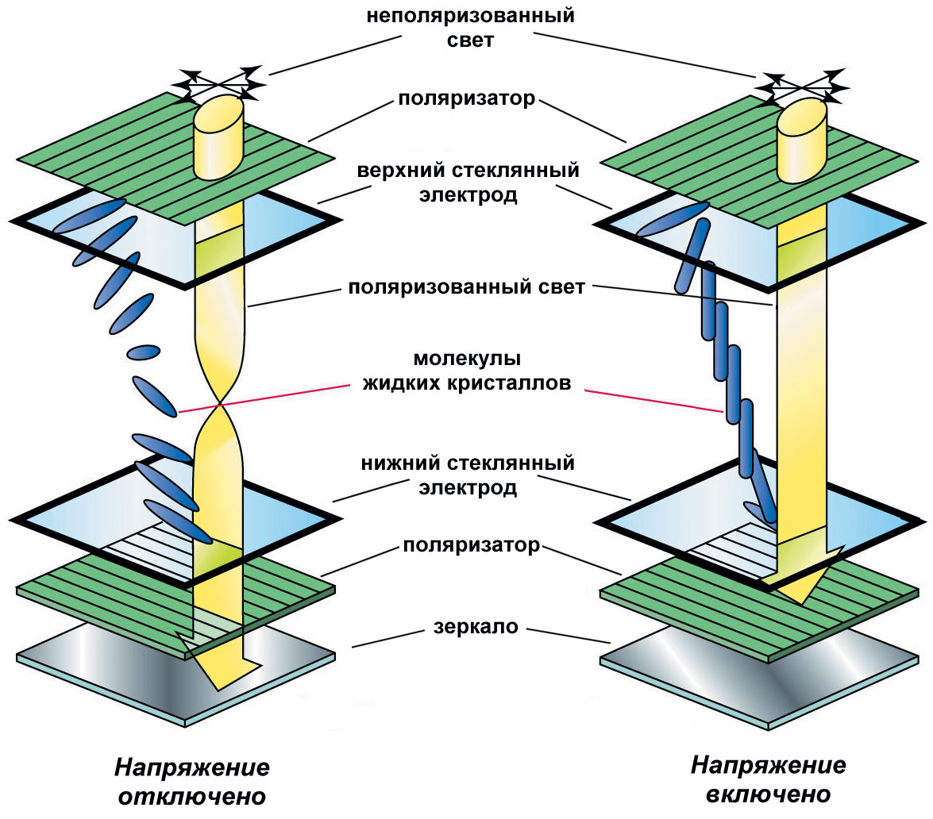
\includegraphics[width=1\textwidth]{12twist.png}
	\label{pic:12twist}
\end{figure}

\textit{Трансмиссивные ЖКИ} (transmissive LCD) используют те же принципы, но фон или сегменты становятся ярче за счет использования задней подсветки.

ЖК-индикаторы на твист-эффекте имеют преимущества по сравнению с ЖК индикаторами на эффекте динамического рассеяния (меньше рабочие токи 1-3 $ \text{мкА}/\text{см}^2 $ вместо 10 $ \text{мкА}/\text{см}^2 $, и поэтому большую долговечность). Быстродействие ЖК на твист-эффекте гораздо выше, чем при использовании динамического рассеяния.

К недостаткам ЖК-индикаторов на твист-эффекте относится меньший, чем у индикаторов на эффекте динамического рассеяния, угол обзора, что связано с узкой диаграммой направленности света при твист-эффекте и влиянием поляризаторов. Применение поляризаторов приводит к потерям до 50~\% света, а также повышает стоимость индикаторов.

Индикаторы без поляризаторов могут быть созданы на основе \textit{эффекта <<гость-хозяин>>}. Современные ЖК в видимой части спектра не имеют собственных полос поглощения, и поэтому к ЖК добавляют небольшое количество дихроичного\footnote{Дихроизм --- различное поглощение веществом света в зависимости от его поляризации (анизотропия поглощения)} красителя (примерно 1-2\% по весу), который имеет собственную полосу поглощения в видимой области спектра электромагнитных волн. В этом случае ЖК-вещество называется <<хозяином>>, а дихроичный краситель называется <<гостем>>. Молекулы <<гостя>> имеют форму сильно вытянутого эллипсоида вращения очень похожую на форму молекул «хозяина». Если ЖК ориентирован каким-либо образом, то и молекулы дихроичного красителя ориентированы точно так же, т.е. стержневидные дихроические молекулы красителя, которые введены в ЖК-вещество, стремятся ориентироваться параллельно осям его молекул. 

В силу того, что молекулы красителя имеют направление преимущественной ориентации точно такое же, как и молекулы ЖК (напомним что, направление преимущественной ориентации молекул ЖК носит название директора), то и вся ЖК-ячейка с дихроичным красителем будет поглощать свет, поляризованный вдоль директора, и не будет поглощать свет, поляризованный перпендикулярно директору. Так как упорядочение длинных осей молекул ЖК и красителя не идеально, то в целом такая ЖК-ячейка будет поглощать свет, поляризованный вдоль директора и перпендикулярно к нему с различными коэффициентами экстинкции. В начальном состоянии, при нулевом напряжении на ЖК-ячейке, свет с любым направлением поляризации поглощается (рис.~\ref{pic:12liquid2}~а), но с различными коэффициентами экстинкции (в зависимости от поляризации).

\begin{figure}[h!]
%	\caption{ Работа ЖК-ячейки на эффекте <<гость-хозяин>> при напряжениях:\\ а -- нулевом; б -- превышающем пороговое;\\ 1 -- молекулы красителя; 2 -- молекулы ЖК }
	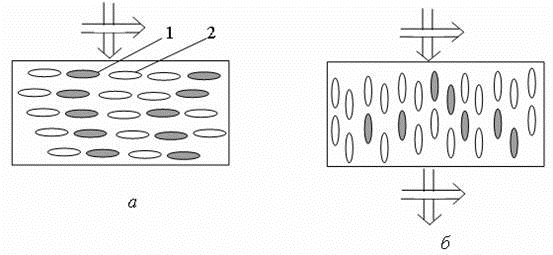
\includegraphics[width=0.6\textwidth]{12liquid2.png}
	\label{pic:12liquid2}
\end{figure}

При наложении на ячейку достаточно сильного электрического поля жидкий монокристалл переориентируется директором вдоль поля, увлекая за собой молекулы красителя (рис.~\ref{pic:12liquid2}~б). Таким образом, управляя ориентацией ЖК, можно регулировать прохождение света. 

Описанная система перспективна, так как позволяет получить почти черное позитивное изображение на белом фоне при высокой яркости и достаточно широком угле обзора. Контраст у индикаторов на эффекте <<гость-хозяин>> несколько хуже вследствие поглощения света красителем.

Эффект <<гость-хозяин>> в ЖК может наблюдаться как при освещении ЖК-ячейки естественным светом, так и при освещении его поляризованным светом. В последнем случае контраст будет выше. При этом входной поляризатор должен быть ориентирован так, чтобы ось максимального пропускания была параллельна ориентации молекул ЖК. Если эффект «гость-хозяин» наблюдать в лазерном свете, то входной поляризатор не требуется.

Угол обзора зависит также от толщины слоя ЖК. Большинство ЖКИ изготавливаются по второму классу с толщиной от 6 до 8 мкм. Первый класс имеет толщину от 3 до 4 мкм. Наиболее широкий угол обзора (до 165$ ^\circ $) достигается при 4-х микронной технологии. При этом также уменьшается время отклика (срабатывания) ЖКИ.

Конструктивно цифровые устройства на жидких кристаллах выполняют в виде конденсатора, между пластинами~3 которого находится слой жидкого кристалла~5 (рис.~\ref{pic:12condensator}) толщиной 10$ \ldots $20~мкм. На внутренние поверхности пластин наносят электроды~4, например из окиси олова, на выводы~1 которых подают управляющее напряжение. Пластины в сборе герметизируют со всех сторон прокладками~2 или помещают в герметизированный корпус. 

\begin{figure}[h!]
	\caption{ Конструкция цифрового устройства на жидких кристаллах }
	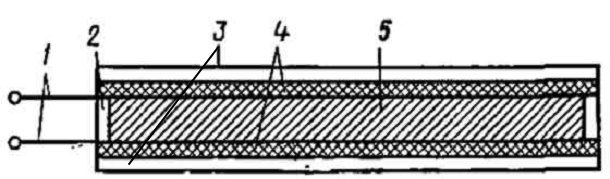
\includegraphics[width=0.5\textwidth]{12condensator.png}
	\label{pic:12condensator}
\end{figure}

\begin{flushleft}
\textbf{Температура использования и хранения}
\end{flushleft}

Анализ температурного диапазона очень важен при описании ЖКИ. Все ЖК материалы имеют строго определенный верхний предел рабочей температуры, или изотропический предел. Выше этого предела молекулы ЖК принимают произвольную ориентацию. Изотропические условия делают позитивное изображение полностью темным, а негативное -- прозрачным. Изотропическая температура называется температурой нематическо-изотропического перехода, или $ N-I $ перехода. 

ЖКИ могут восстанавливаться после короткого воздействия изотропической температуры, хотя температуры свыше 110$ ^\circ $C разрушают внутреннее покрытие индикатора. 

Нижний предел температурного диапазона ЖКИ не так хорошо определен, как верхний. При низких температурах время срабатывания индикатора увеличивается, так как замедляется движение молекул и возрастает вязкость ЖК вещества. 

При очень низких температурах ЖК вещество переходит в твердое, или кристаллическое состояние. Эта температура называется температурой кристаллическо-нематического перехода, или $ C-N $ перехода. Однако ЖК материал <<суперхолодный>>, воспринимает температуры ниже $ C-N $ предела, фактически поворачивая кристаллы вещества. (Обычно при воздействиях до $-60 ^\circ $C). В результате ЖКИ часто работоспособны при температурах ниже их $ C-N $ перехода.

Эффект низких температур обычно обратим. К примеру, ЖКИ опущенный в жидкий азот возвращается в нормальное состояние после короткого периода нагрева. 

В добавление, ЖК материалы имеют низкий температурный коэффициент. Этот коэффициент важен для мультиплексных индикаторов по причине низкого значения действущего напряжения управления. За пределами температурного диапазона может потребоваться температурная компенсация.

Достоинства ЖК-индикаторов заключаются в следующем:
\begin{itemize}
\item малая потребляемая мощность (110 $ \text{мкВт}/\text{см}^2 $);
\item работа при высоком уровне внешней освещенности;
\item простота конструкции и технологии изготовления;
\item низкая стоимость, низкое рабочее напряжение.
\end{itemize}

К основным недостаткам ЖК-индикаторов следует отнести:
\begin{itemize}
\item узкий диапазон рабочих температур (от $ -10 $ до $ +60^\circ $С);
\item длительные переходные процессы, к тому же зависящие от температуры.
\end{itemize}

\section{Плазменная индикаторная панель}

Плазменная технология --- передовой шаг в развитии и производстве индикаторных экранов, панелей, табло. Результатом данной технологии является богатая и точная передача цветовой гаммы на большом экране толщиной всего несколько сантиметров. 

\textit{Плазменная панель} (газоразрядный экран) --- устройство отображения информации основанное на явлении свечения люминофора под воздействием ультрафиолетовых лучей, возникающих при электрическом разряде в ионизированном газе, иначе говоря, в плазме. Рассмотрим подробнее физический принцип работы и технологию, применяемые при изготовлении плазменных панелей.

Еще в девятнадцатом веке стал известен процесс холодного газового разряда, который впоследствии применили во всем хорошо известных неоновых лампах. В плазменных панелях применяется тот же принцип, только такие лампы чрезвычайно малы, и газ это не всегда неон. Чтобы понять, как работают плазменные технологии и получается изображение на экране плазменной панели, давайте вернемся к неоновым лампам (рис.~\ref{pic:12plasma}):

\begin{figure}[h!]
	\caption{ Схема работы плазменной технологии на основе газоразрядной трубки }
	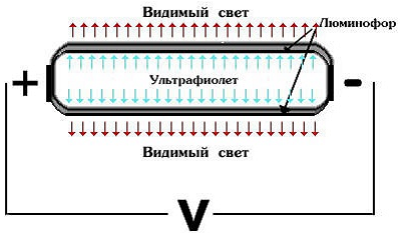
\includegraphics[width=0.65\textwidth]{12plasma.png}
	\label{pic:12plasma}
\end{figure}

Имеется запаянная стеклянная трубка (капсула), внутри которой заключен инертный газ, такой как неон, аргон или смесь разных газов, кроме него в трубке находятся пары какого либо тяжелого металла. По обеим сторонам трубки расположены электроды, на которые подается напряжение, под воздействием тока у заполняемого трубку газа высвобождаются свободные электроны, образуется  холодная плазма, состоящая из положительно заряженных ионов газа и  электронов. Далее начинается движение частиц плазмы: электронов к положительно заряженному электроду, ионов к отрицательно заряженному. 

В результате движения частицы плазмы сталкиваются с атомами тяжелого металла, в результате столкновений эти атомы набирают энергию и их электроны переходят на более высокую орбиту. При переходе электронов атома на прежнюю орбиту высвобождаемая энергия образует фотон, то есть квант света. При этом испускаемый свет – это невидимый человеческим глазом ультрафиолет. Для его визуализации служит слой люминофора, превращающий ультрафиолет в видимый свет, такой свет может быть любого цвета. Есть еще одна проблема, что будет, когда все частицы плазмы перетекут к своим электродам? Для того чтобы движение не останавливалось, к электродам применяют переменное напряжение. Получается так, что плазма постоянно меняет свое направление движения, не прекращая его. 

Для того чтобы получить точку нужного нам цвета недостаточно одной газоразрядной капсулы, поэтому пиксель на PDP состоит из трех таких капсул (рис.~\ref{pic:12pixel}): красной, зеленой и синей. Эти капсулы составляют RGB (red, green, blue) триаду внутри каждой из них заключено вещество люминофора, испускающее только один из этих основных цветов, другие требуемые оттенки получаются за счет их смешения. 

Плазменная панель представляет собой матрицу газонаполненных ячеек, заключенных между двумя параллельными стеклянными пластинами, на внутренних поверхностях которых нанесены прозрачные электроды, образующие соответственно шины сканирования, подсветки и адресации.

\begin{figure}[h!]
	\caption{ Схема плазменной ячейки (пикселя) }
	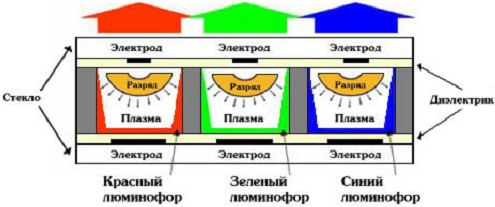
\includegraphics[width=0.5\textwidth]{12pixel.png}
	\label{pic:12pixel}
\end{figure}

Разряд в газе протекает между разрядными электродами (сканирования и подсветки) на лицевой стороне экрана и электродом адресации на задней стороне. Яркость каждого элемента изображения определяется временем свечения соответствующей <<ячейки>> плазменной панели: самые яркие элементы <<горят>> постоянно, а в наиболее темных местах они вовсе не <<поджигаются>>. Светлые участки изображения на PDP светятся ровным светом, и поэтому изображение абсолютно не мерцает. Подавая управляющие сигналы на вертикальные и горизонтальные электроды (нанесенные на внутренние поверхности стекол панели) схема управления PDP осуществляет соответственно вертикальную и горизонтальную развертку растра изображения.

Современные плазменные панели позволяют производить просмотр изображений на них под углом до 160$ ^\circ $ к экрану. Яркость плазменной панели такова, что смотреть ее можно при любом свете – огромный плюс по сравнению с проекторами, для которых яркость освещения помещения всегда является критичной. Плазменная панель не создает вредных магнитных и электрических полей, так как в ней отсутствует устройство развертки и высоковольтный источник анодного напряжения (как в кинескопе). Плазменная панель также не оказывает вредного влияния на человека и домашних животных и не притягивает пыль к поверхности экрана. Кроме того, что очень важно, плазменная панель не имеет рентгеновского и какого-либо иного излучения. 

%\section{Сравнение жидкокристаллических и плазменных \\индикаторных устройств}

\begin{flushleft}
\textbf{Контрастность изображения}
\end{flushleft}

Плазменная технология добилась значительных успехов в разработке изображений повышенной контрастности. Для того, чтобы сформировать тёмные или чёрные пиксели, в плазменной технологии просто блокируется подача энергии (посредством сложных внутренних алгоритмов) на определенные пиксели. Нанося время от времени вред формированию полутонового изображения, эта методика действительно даёт тёмные чёрные цвета. В LCD технологии, напротив, нужно увеличивать подачу энергии, чтобы сделать пиксели более тёмными. 

Поэтому чем большее напряжение подаётся на пиксель и проходит через него, тем темнее становится LCD-пиксель. Несмотря на достигнутые в LCD технологии некоторые улучшения контрастности и уровня чёрного цвета контрастность плазменных индикаторных устройств выше. 

Преимущество имеет плазменная панель. 

\begin{flushleft}
\textbf{Насыщенность цвета}
\end{flushleft}

Цветовая информация более точно реализовывается и воспроизводится в плазменных панелях, поскольку вся информация, необходимая для показа любого спектрального цвета, содержится в каждой пиксельной ячейке. Каждый пиксель содержит синий, зелёный и красный элементы для точной и детальной передачи цвета. Насыщенность, являющаяся результатом пиксельной структуры плазменной панели, обеспечивает самые живые цвета среди любого типа экранов. Координаты цветности на хороших плазменных панелях намного более точны, чем на LCD. Цветовая информация имеет преимущество вследствие меньшего размера пиксельной матрицы большинства LCD-телевизоров. Однако при одинаковом размере пикселя цвет будет не таким выразительным, как у плазменных панелей.

Преимущество имеет плазменная панель, с большим запасом. 

\begin{flushleft}
\textbf{Долговечность}
\end{flushleft}

Производители LCD утверждают, что долговечность их мониторов/телевизоров составляет от 50~000 до 75~000 часов. LCD-монитор может работать столь же долго, сколько работает лампа подсветки (которую в действительности можно заменять), так как свет от неё, подвергаясь воздействию жидкокристаллической призмы, обеспечивает яркость и цвет. С другой стороны, в плазменной технологии на каждый пиксель подаётся небольшой электрический импульс, который возбуждает редкие инертные газы~--- аргон, неон и ксенон (в конце цепочки~-- люминофоры), необходимые для обеспечения цвета и яркости. Эти инертные газы в действительности имеют срок жизни и со временем их ядра подвергаются распаду. Изготовители плазмы оценивают долговечность люминофоров и, следовательно, самих панелей в 25~000~-- 30~000 часов. Люминофоры не могут быть заменены. Не существует также такого явления, как закачка новых газов в плазменный дисплей. 

Преимущество имеет LCD, в два и более раза. 

\begin{flushleft}
\textbf{Выжигание экрана}
\end{flushleft}

Для LCD можно не учитывать факторы, приводящие к выжиганию экрана при проецировании статических изображений. У плазменной технологии, напротив, следует учитывать факторы, приводящие к выжиганию экрана при отображении статической картинки. Статические изображения начнут выжигать отображаемую картинку через короткий промежуток времени -- в некоторых случаях спустя примерно 15 минут. Хотя выжигание можно обычно отмыть, используя серые изображения или непрерывные полноцветные диапазоны в течение нескольких часов, оно, тем не менее, является значительным фактором, препятствующим развитию плазменной технологии. 

Преимущество имеет LCD экран. 

\begin{flushleft}
\textbf{Использование вместе с компьютером}
\end{flushleft}

LCD отображает статические изображения от компьютера эффективным образом и с полной цветовой гаммой, без мерцаний и выжигания экрана. Плазменной панели труднее обрабатывать статические изображения от компьютера. Хотя их отображение выглядит удовлетворительным, проблемой является выжигание экрана; представляет трудность и шаговый эффект, встречающийся в панелях с меньшей разрешающей способностью при отображении статических надписей (Power Point). Видеоизображения с компьютера получаются качественными, но возможно некоторое мерцание, зависящее как от заводского качества панели, так и от отображаемого разрешения. Плазменная панель выигрывает по углу обзора. 

Преимущество имеет LCD, за исключением больших углов обзора.

\begin{flushleft}
\textbf{Воспроизведение видео}
\end{flushleft}

Здесь следует отдать должное плазменной панели, поскольку она имеет прекрасное качество при отображении сцен с быстрым движением, высококонтрастные уровни, цветовую насыщенность и яркость. На LCD будет заметен эффект трейлера во время показа сцен с быстрым движением от видео, так как эта технология медленнее реагирует на изменения цвета. У LCD также более низкие уровни контрастности.

Преимущество имеет плазменная панель.

\begin{flushleft}
\textbf{Требования по напряжению}
\end{flushleft}

У LCD технологии гораздо меньшие требованию по напряжению, чем у плазменных панелей. С другой стороны, при использовании плазменной панели необходимым (трудновыполнимым) условием является подача энергии на сотни тысяч прозрачных электродов, которые дают свет и возбуждают заключённые в каждой ячейке пикселя люминофоры. 

Преимущество имеет LCD панель.

\begin{flushleft}
\textbf{Использование в нестандартых условиях}
\end{flushleft}

В принципе, нет ничего, что служило бы препятствием для размещения LCD монитора на высокогорье, как и нет никаких реальных ограничений. Этим объясняется использование LCD экранов в качестве главного обзорного экрана для отображения видеоинформации о полётах. Поскольку ячейка плазменного экрана в плазменных панелях в действительности является стеклянной оболочкой-субстратом, содержащей редкие инертные газы, то разреженный воздух приводит к увеличению давления в газах, находящихся внутри этой оболочки. Это вызывает перерасход энергии, требуемой для запуска и охлаждения плазменной панели, в результате чего усиливается гудение (жужжание) или появляется шум от вентилятора. Эти проблемы возникают на высоте приблизительно 2000~м. 

Преимущество имеет LCD панель.
